%!TEX root = ../main.tex

\section{Numerical studies}

In this section we present some numerical results
obtained using finite-difference
scheme~\eqref{sch:transition},\eqref{sch:borders},
presented above. The main goal of the simulations is to confirm
theoretical stability estimates derived for the model itself and its
approximations,
i.e.,~--- convergence and stability  of the finite-difference scheme
(see section~\eqref{cond:spectral_better})
and
stability properties of the equilibrium solutions
described in section~\ref{sec:theoretical_analysis}.
Besides this we will check temporal behaviour of the
total free energy of the system.

\subsection{Typical solution}

Let us set the parameters of the equation~\eqref{eq:one_dim} as follows:
\begin{equation}
	\epsilon_0 = 0.2, \; \delta = 0.04, \; l = 1.0, \; \Gamma = 1.0, \; m = 0.5, \; K_\Phi = 4.8 \tpoint
	\label{exp:parameters}
\end{equation}
Note that this set of parameters corresponds to the ``strong electric
field'' case, see~\eqref{char:equilibriums}.

The equation is solved in spatiotemporal domain
\begin{equation}
	\clOmega = [0, W]_x \times [0, T]_t, \; W = 5, \; T = 1 \tpoint
	\label{exp:set}
\end{equation}

Boundary conditions are defined as follows:
\begin{equation}
\begin{gathered}
  \phi(0, t) = 1, \; \phi(W, t) = 1 \tcomma \\
  \phi(x, 0) = \phi_0(x) = \begin{cases}
    1, \; \text{if} \; x \leqslant 2.25 \; \text{or} \; x \geqslant 2.75 \tsemicolon \\
    1 - 0.025 \cdot [1 + \cos(4 \pi x)], \; \text{if} \; 2.25 < x < 2.75 \tpoint
  \end{cases}
\end{gathered} \label{exp:borders}
\end{equation}
Note that~$\phi_0(x)$ is a twice differentiable function everywhere
except finite number of points; more over, its second derivative is bounded.

Let~$N_x$ be the number of grid steps on~$[0, W]_x$ (the number of
nodes is, respectively,~$N_x + 1$);
$N_t$~--- be the number of mesh steps on~$[0, T]_t$.
Spatial and temporal mesh step sizes are given by~$h = W / N_x, \; \tau = T / N_t$.

On Fig.~\ref{fig:typical_solution} the typical solution is presented.
It easy to see gradual evolution of the breakdown channel
(identified as a spatial domain where medium is damaged)
staring from the sufficiently small perturbation
of the initial, completely undamaged, state.
Approximately at time~$t = 0.55$ the medium in the breakdown channel
becomes completely damaged: the values of~$\phi$ in the neighborhood
of~$x = 2.5$
is closed to zero value.
Note that for~$t \in (0.3, \; 0.55)$ the breakdown channel
(identified as a spatial domain where~$\phi$ essentially differs from~1)
practically doesn't change its width which is equal approximately
to~$2l$, as supposed by the model. In turn, for~$t > 0.55$
when~$\phi$  reaches its minimal values, it start to
grow wide with almost constant velocity.


\subsection{Evolution of free energy}

In the model under consideration, the free energy of the system is given
by~\eqref{eq:energy} with its density given by~\eqref{eq:energy_density}.
In finite-dimensional setting, the terms in~\eqref{eq:energy_density}
are approximated in the obvious way. 
The only essential addition we need to mention is approximation of
first derivative, i.e., 
$\partial_h \phi_i^j / \partial_h x$.
Further the simplest approach is considered which uses standard
1st-order approximation of~$\partial_h \phi_i^j / \partial_h x$.

To simulate solution of the system, we use the same
finite-difference scheme, initial and boundary conditions as in the
previous section.

The results are given in Fig.~\ref{fig:energy} where
dependence~$\Pi = \Pi(t)$ is shown.
The colored vertical dashed lines correspond to the same moments of time as on Fig.~\ref{fig:typical_solution}. 
It is interesting to note that for~$t < 0.5$ free energy~$\Pi$ is
almost constant; further, for~$t > 0.5$ it starts to decrease
sufficiently fast until~$t \approx 0.55$. Later, after~$t = 0.6$ the
energy decreases linearly, until the complete damage of the medium.

\begin{figure}[!p]
  \centering
  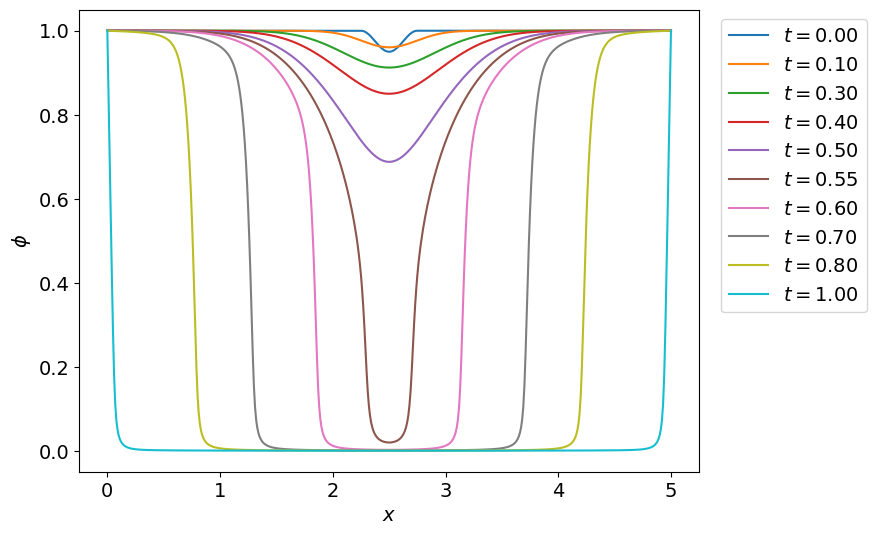
\includegraphics[width=\textwidth]{figures/typical_solution.png}
  \vspace{-0.8cm}
  \caption{Typical solution of the problem, $N_x = 10^3$, $N_t = 10^5$.}
  \label{fig:typical_solution}
  
  \vspace{1.5cm}
  
  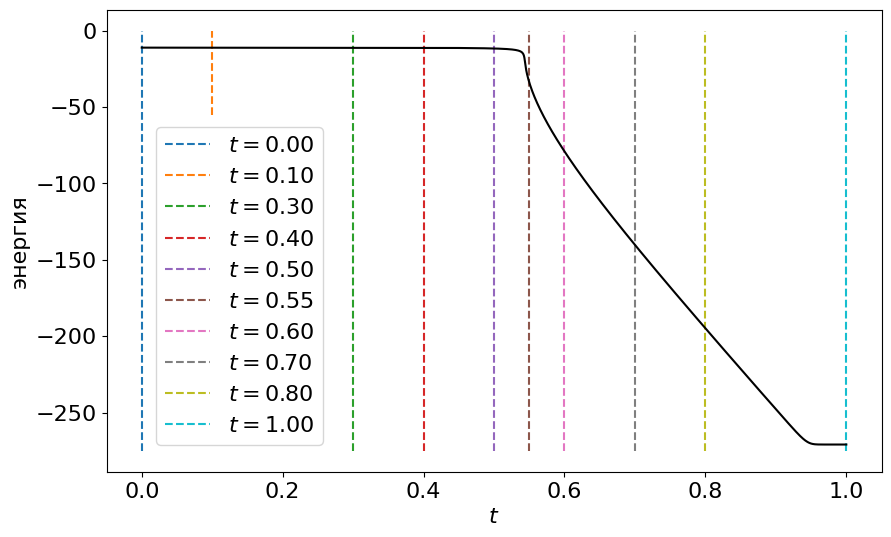
\includegraphics[width=\textwidth]{figures/energy_total.png}
  \caption{Free energy evolution.}
  \label{fig:energy}
\end{figure}

It can be seen from the derivation of~\eqref{eq:phi:a} and~\eqref{eq:phi:b},
that during its evolution, the system tends to minimize its free energy.
Due to this, the correct monotone evolution of free energy
is of the crucial importance for simulation to be qualitatively correct.
We do not provide here the strict proof of the correct behavior of the
scheme (which is an important, but standalone task), but rather check
it in the performed simulations. This means that under given
parameters of the model and discretization, the scheme is
gradient-stable (or, which is same, energy stable).


\subsection{Stability of the scheme}

In this section we check stability
estimate~\eqref{cond:spectral_better} of the
finite-difference scheme.

Let the model parameters be defined according
to~\eqref{exp:parameters} and~\eqref{exp:set}, boundary conditions are given by~\eqref{exp:borders}.
We assume by convention that the scheme is unstable as soon as
the simulation finishes abnormally with floating point overflow
due to division by zero (e.g., in expression~\eqref{eq:epsilon}
for~$\epsilon(\phi)$
at~$f(\phi) = -\delta$)
or values of~$\phi$ go to infinity
(as in overflow of  variables of the type~\texttt{double}).
We then increase~$N_x$ and~$N_t$, keeping information about
pairs of values at which stable approximation turns into unstable one.
Plotting these values we can depict stability region of the scheme
on the~$N_x$--$N_t$ plane.
Such plot is presented on Fig.~\ref{fig:stability_bounds}
together with theoretical boundary given by the stability
estimate~\eqref{cond:spectral_better}.

Numerical experiment demonstrates that the
estimate~\eqref{cond:spectral_better} is successful and sufficiently
sharp: theoretical and experimental stability boundaries follows each other and
are relatively closed. Moreover, the theoretical curve lies above
the experimental one which means that theoretical estimate is more
strict then the experimental one. Actually this was a reason divide
right hand side of the original estimate~\eqref{cond:spectral_better_theoretical} by two.
\begin{figure}[!t]
	\centering
	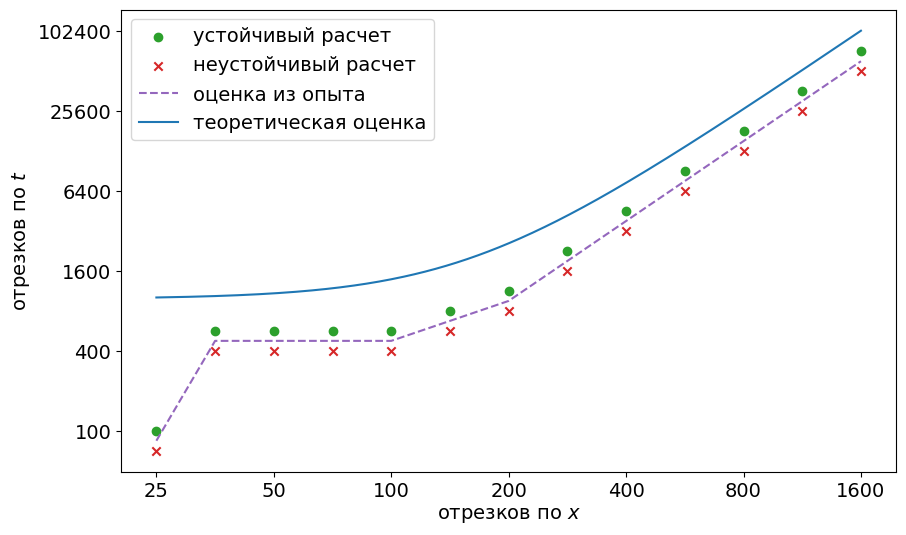
\includegraphics[width=\textwidth]{figures/stability_bounds.png}
	\vspace{-0.7cm}
	\caption{Theoretical and experimental stability boundaries.}
	\label{fig:stability_bounds}
\end{figure}


\subsection{Convergence}

Approximation property of the finite-difference scheme~\eqref{sch:transition},
\eqref{sch:borders} for solution of~\eqref{eq:one_dim},
\eqref{eq:one_dim_initial} and~\eqref{eq:one_dim_marginal} is obvious.
Stability of the scheme is provided by the theoretical
estimate~\eqref{cond:spectral_better}, which was
verified against numerical experiments.
We now check convergence of the finite-difference solution.

Define~$\enorm_C$ and~$\enorm_2$ norms as
$$\norm{f}_C = \max \limits_{(x, t) \in \clOmega} |f(x, t)|; \qquad \norm{f}_2 = \sqrt{\int \limits_{\clOmega} f^2(x, t) dx dt} \tpoint$$
on the space~$C_2(\clOmega)$ of twice differentiable functions in the
closed spatiotemporal domain~$\clOmega = [0, W]_x \times [0, T]_t$.

Assume that computational mesh~$\Omega_{h, \tau} \subset \clOmega$
together with some dependence~$\tau = \tau(h)$.
Restricting functions from~$C_2(\Omega)$ on the mesh~$\Omega_h =
\Omega_{h, \tau(h)}$, we obtain a space of mesh functions~$C_2(\clOmega)_h$.
Functional norms in the space~$C_2(\clOmega)_h$ can be defined as
$$\norm{f_j^k}_C = \max \limits_{(j, k) \in \Omega_h} |f_j^k|; \qquad \norm{f_j^k}_2 = \sqrt{h \tau \sum \limits_{(j, k) \in \Omega_h} (f_j^k)^2} \tpoint$$

Now consider the results of the numerical experiments.
Convergence will be analysed using norms~$\enorm_C$ и $\enorm_2$
defined on the space of mesh functions defined above.
Since analytical solution of the problem is not known, 
comparison will be performed using a sequence of approximate
solutions
against the solution obtained using the finest
mesh. To compute difference between two finite-difference solutions,
we restrict solution obtained using more fine grid on the more coarse
grid,
ignoring fine solution values at the respective mesh nodes.

To proceed we set the parameters of the model as described above,
see~\eqref{exp:parameters}, \eqref{exp:set}.
Let~$N_x = W / h$ be the number of mesh steps in spatial domain,
$N_t = T / \tau$ be the number of mesh steps in time domain.
In all simulations stability condition~\eqref{cond:spectral_better} is
satisfied.

First, we set~$N_x = 200$ and perform a sequence  of simulations with
gradually increasing~$N_t$, doubling it at each step.
Comparison of the obtained solutions with the one obtained for~$N_t =
204800$ is shown in Fig.~\ref{fig:convergence_fixed_nx}.
Simulated results clearly shows that the scheme produces solutions
with first order convergence rate to the ``exact'' one in time~$t$ which
confirms theoretical estimates; the scheme has~$\bigO (\tau)$ accuracy.

Second, we set~$N_t = 204800$ perform a sequence  of simulations with
increasing~$N_x$, again, doubling it at each step.

Comparison of the obtained solutions with the one obtained for~$N_x = 1600$
is shown in Fig.~\ref{fig:convergence_fixed_nt}.
Simulated results clearly shows that the scheme produces solutions
with second order convergence rate to the ``'exact'' one in spatial variable~$x$ which
confirms theoretical estimates; the scheme has~$\bigO (h^2)$ accuracy.

\begin{figure}[!tp]
	\centering
	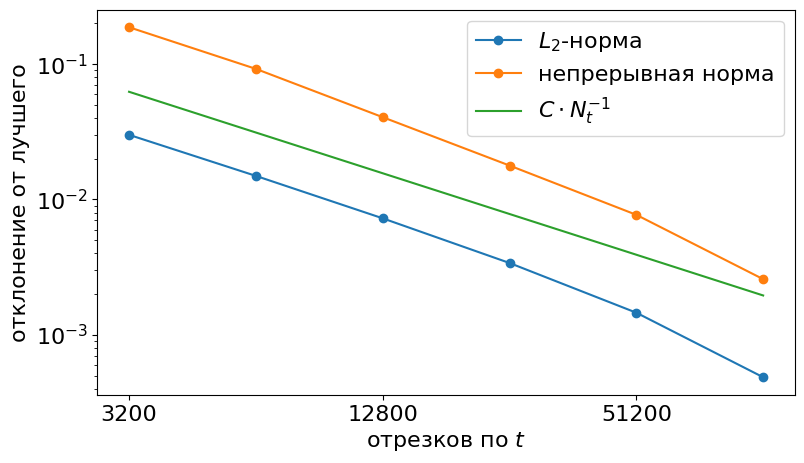
\includegraphics[width=0.79\textwidth]{figures/convergence_fixed_nx.png}
	\vspace{-0.2cm}
	\caption{Error norm for fixed~$N_x = 200$.}
	\label{fig:convergence_fixed_nx}
	\vspace{0.6cm}
	
	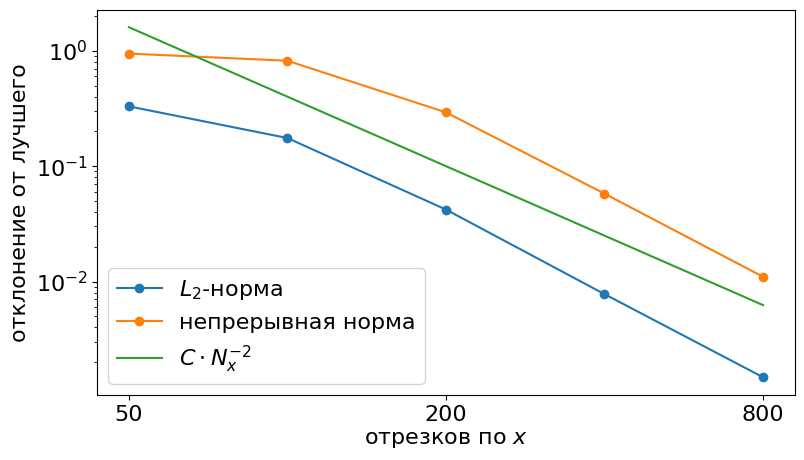
\includegraphics[width=0.79\textwidth]{figures/convergence_fixed_nt.png}
	\vspace{-0.2cm}
	\caption{Error norm for fixed~$N_t = 204800$.}
	\label{fig:convergence_fixed_nt}
	\vspace{0.6cm}
	
	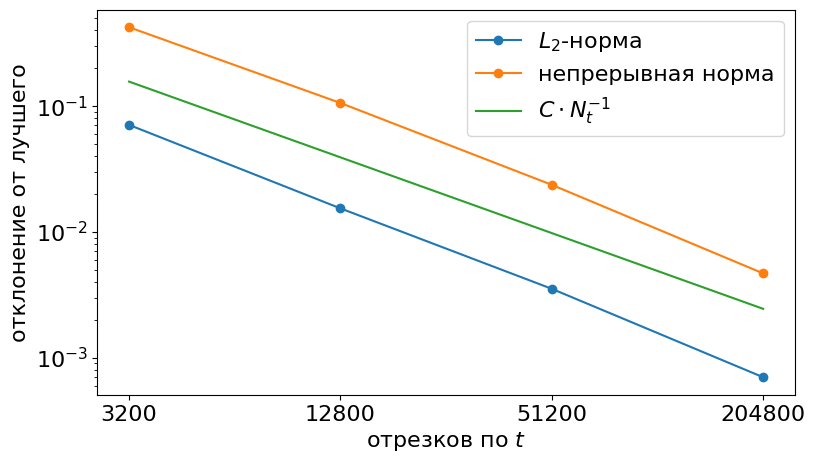
\includegraphics[width=0.79\textwidth]{figures/convergence_connected.png}
	\vspace{-0.2cm}
	\caption{Error norm for~$N_t = 0.08 \cdot N_x^2$.}
	\label{fig:convergence_connected}
\end{figure}

We now refine both~$N_x$ and~$N_t$ in such a way that for the given
values of~$h$ and~$\tau$ ~$h, \tau \to 0$ it holds stability
condition~\eqref{cond:spectral_better}.
For the parameters of the model defined above, one can set~$N_t = 0.08
\cdot N_x^2$.
Computations of the errors between a sequence of approximate solutions and the reference one is
performed in the same way as earlier; the results are presented on
Fig.~\ref{fig:convergence_connected}.
As it is expected, the convergence order is~$\bigO (\tau + h^2) =
\bigO (\tau)$ as soon as spatial and temporal discretization
parameters are related as described above.

Note that in the first two experiments, the limiting solution was not
actual
solution of the differential problem since only one discretization
parameter was tending to its limiting value. The second one
had the fixed value and, therefore, reference numerical solution
always had irremovable approximation error.
In the third experiment, under assumption that the scheme is stable,
numerical solutions converges to the solution of the initial
differential problem~\eqref{eq:one_dim}, \eqref{eq:one_dim_initial}, \eqref{eq:one_dim_marginal}.


\subsection{Stability of the equilibrium states}

Earlier we studied equilibrium solutions~$\phi \equiv C$ of the
equation~\eqref{eq:one_dim}.
Their number and stability type are defined by the value of
the parameter~$\xi$ given by~\eqref{char:equilibriums}.

Define parameters of the model according to~\eqref{exp:parameters}
and~\eqref{exp:set},~---
except the value of~$K_\Phi$  which will be defined later.
As the  initial condition, we set perturbation of the constant
equilibrium state:
$\phi(x, 0) = C + A \cos(\omega x); \; \phi(0, t) = \phi(0, 0), \;
\phi(W, t) = \phi(W, 0)$.
The amplitude~$A$ is considered to be relatively small, i.e.,~$A\sim0.01$.
A number of computational steps is given by~$N_x = 800$ and~$N_t = 51200$.

If the equilibrium state is stable, then for an arbitrary~$\omega$
perturbations in the initial condition decay;
if the equilibrium state is unstable, then there exists
some~$\omega_0$,
such that for any~$\omega < \omega_0$ perturbations increase in time.

Let us set~$K_{\Phi, 1} = 0$, $K_{\Phi, 2} = 1.1$, $K_{\Phi, 3} =
4.8$. For~$\delta = 0.04$, as it was defined above,
one has~$\xi_1 = 0 < \delta^2$,
$\xi_2 = 0.121 \in (\delta^2, (1+\delta)^2)$, $\xi_3 = 2.304 > (1 + \delta)^2$.

First, consider~$K_{\Phi, 1} = 0$, $\xi_1 < \delta^2$~---
which is the case of ``weak electric field''.
In this case the system has two equilibrium states:
$\phi \equiv 0$~--- the unstable one and~$\phi \equiv 1$~--- the
stable one.
On the Figs.~\ref{fig:equilibrium_1_0} and~\ref{fig:equilibrium_1_1}
it is easy to see theoretically predicted evolution of the solution:
for~$C = 0$ perturbations  growth, for~$C = 1$~--- perturbation
decreases.
For value~$C = 0$ derivative of the function~$\chi(\phi)$
(see~\eqref{eq:equilibruim_characteristic}) vanishes, therefore,
to observe growth of perturbations, it is necessary to define
sufficiently small values of~$\omega$,
which, in turn, provides sufficiently small
value of~$\partflxx{\phi}$.
Note that in the experiment with~$\phi \equiv 1$,
we take~$C = 1 - A$, in order to keep the values of~$\phi$ below~$1$.

\begin{figure}[!t]
	\centering
	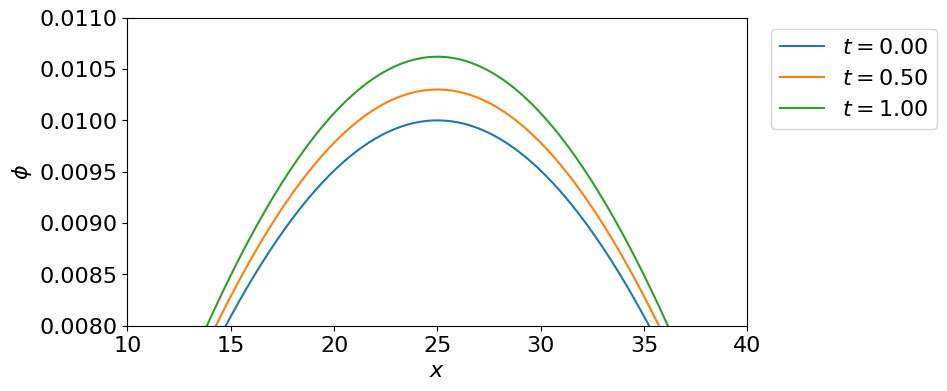
\includegraphics[width=0.99\textwidth]{figures/equilibrium_1_0.png}
	\vspace{-0.3cm}
	\caption{``Weak electric field'' case: perturbed equilibrium state~$\phi \equiv 0$, unstable.}
	\label{fig:equilibrium_1_0}
	\vspace{0.5cm}
	
	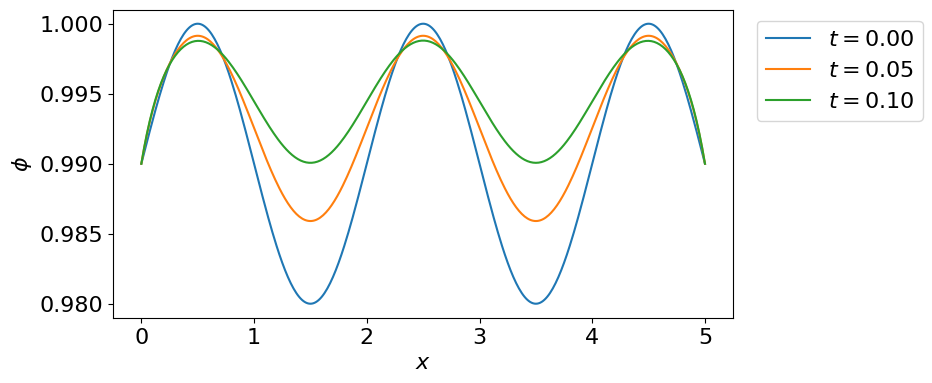
\includegraphics[width=0.99\textwidth]{figures/equilibrium_1_1.png}
	\vspace{-0.3cm}
	\caption{``Weak electric field'' case: perturbed equilibrium state~$\phi \equiv 1$, unstable.}
	\label{fig:equilibrium_1_1}
\end{figure}

Consider now~$K_{\Phi, 2} = 1.1$, $\xi_2 \in (\delta^2, (1 +
\delta)^2)$~--- i.e., the case of ``medium electric field''.
In this case the system has three equilibrium  states: $\phi \equiv
0$~--- stable, $\phi \equiv C_3 \approx 0.5$~--- unstable ($C_3$ is a
zero of~$\chi(\phi)$ in the interval~$(0, 1)$), $\phi \equiv 1$~---
stable.
Evolution of the perturbed solution is shown on
Figs.~\ref{fig:equilibrium_2_0}, \ref{fig:equilibrium_2_05}
and~\ref{fig:equilibrium_2_1}.
As it can be seen, the observed behavior is in accordance with the
theoretically predicted one.

\begin{figure}[!tp]
  \centering
  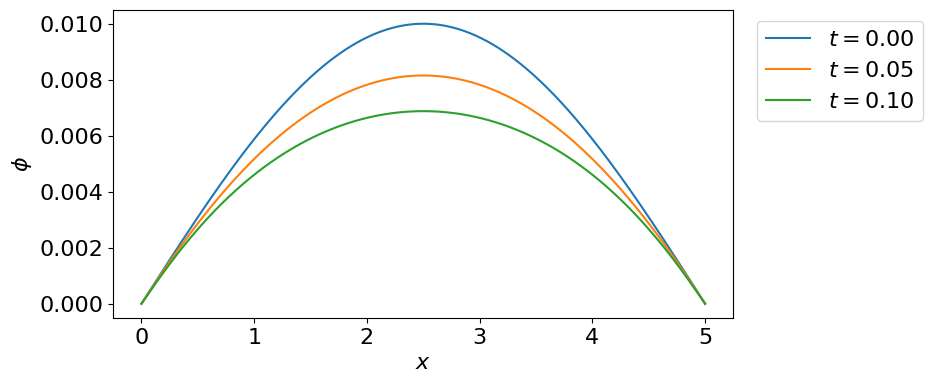
\includegraphics[width=0.99\textwidth]{figures/equilibrium_2_0.png}
  \vspace{-0.3cm}
  \caption{``Medium electric field'' case: perturbed equilibrium state~$\phi \equiv 0$, stable.}
  \label{fig:equilibrium_2_0}
  \vspace{0.5cm}
  
  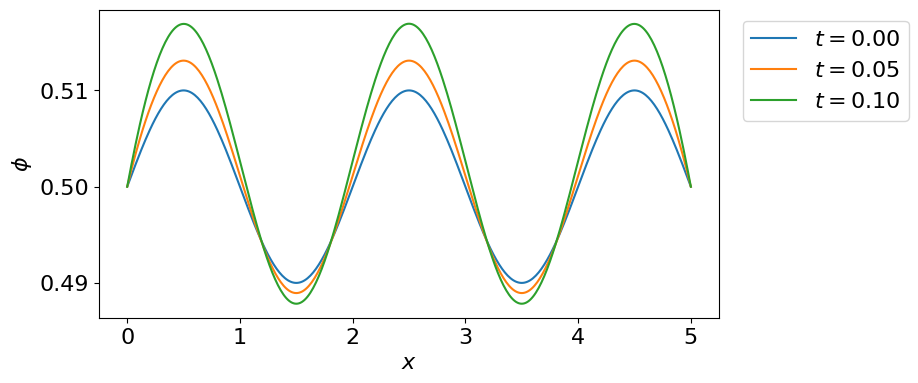
\includegraphics[width=0.99\textwidth]{figures/equilibrium_2_05.png}
  \vspace{-0.3cm}
  \caption{``Medium electric field'' case: perturbed equilibrium~$\phi \equiv C_3 \approx 0.5$, unstable.}
  \label{fig:equilibrium_2_05}
  \vspace{0.5cm}
  
  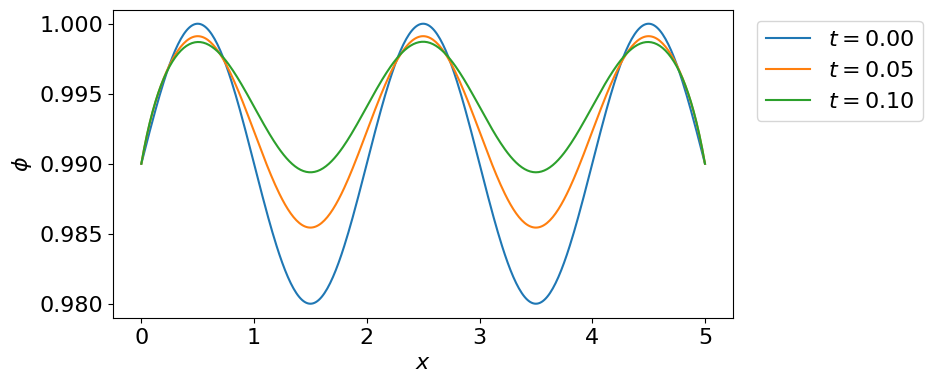
\includegraphics[width=0.99\textwidth]{figures/equilibrium_2_1.png}
  \vspace{-0.3cm}
  \caption{``Medium electric field'' case: perturbed equilibrium state~$\phi \equiv 1$, stable.}
  \label{fig:equilibrium_2_1}
\end{figure}

Finally, consider the case of~$K_{\Phi, 3} = 4.8$, $\xi_3 > (1 +
\delta)^2$~--- which correspond to the ``strong electric field'' case.
The system has two equilibrium states: $\phi \equiv 0$, stable,
and~$\phi \equiv 1$, unstable.
Evolution of the perturbed solution is shown on
Figs.~\ref{fig:equilibrium_3_0} and~\ref{fig:equilibrium_3_1}.
As in other considered cases, the results coincide with the theoretical predictions.

\begin{figure}[!t]
  \centering
  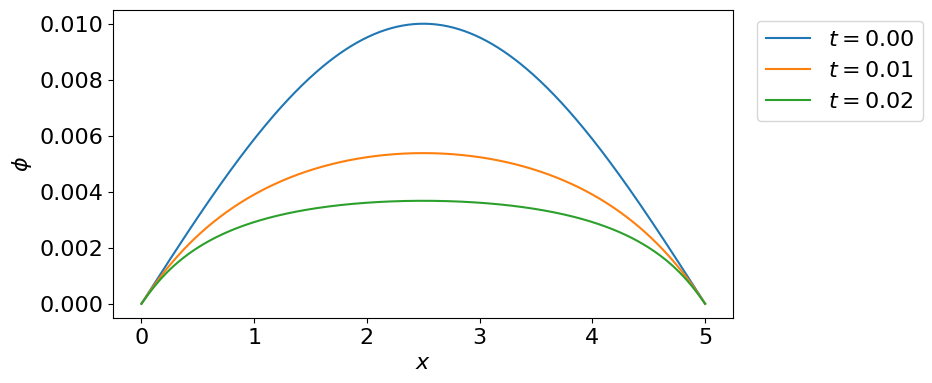
\includegraphics[width=0.99\textwidth]{figures/equilibrium_3_0.png}
  \vspace{-0.3cm}
  \caption{``Strong electric field'' case: perturbed equilibrium
    state~$\phi \equiv 0$, stable.}
  \label{fig:equilibrium_3_0}
  \vspace{0.5cm}
  
  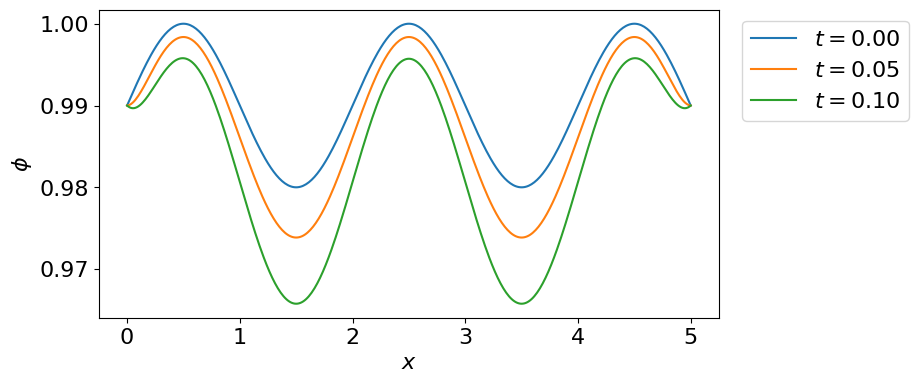
\includegraphics[width=0.99\textwidth]{figures/equilibrium_3_1.png}
  \vspace{-0.3cm}
  \caption{``Strong electric field'' case: perturbed equilibrium
    state~$\phi \equiv 1$, unstable.}
  \label{fig:equilibrium_3_1}
\end{figure}

\endinput
% EOF
